\documentclass[11pt,a4paper]{article}

% ── Packages ──
\usepackage[utf8]{inputenc}
\usepackage[T1]{fontenc}

\usepackage[margin=1in]{geometry}
\usepackage{amsmath,amssymb,amsthm,mathtools}
\usepackage{bm}
\usepackage{graphicx}
\usepackage{xcolor}
\usepackage{hyperref}
\usepackage{listings}
\usepackage{algorithm}
\usepackage{algpseudocode}
\usepackage{booktabs}
\usepackage{enumitem}
\usepackage{tcolorbox}
\usepackage{tikz}
\usepackage{pgfplots}
\pgfplotsset{compat=1.18}

\hypersetup{colorlinks=true,linkcolor=blue!70!black,citecolor=green!50!black,urlcolor=blue!60!black}

% ── Theorem environments ──
\newtheorem{theorem}{Theorem}[section]
\newtheorem{lemma}[theorem]{Lemma}
\newtheorem{proposition}[theorem]{Proposition}
\newtheorem{definition}[theorem]{Definition}
\newtheorem{remark}[theorem]{Remark}
\newtheorem{example}[theorem]{Example}

% ── Code style ──
\lstset{
  language=Python,
  basicstyle=\ttfamily\small,
  keywordstyle=\color{blue!70!black}\bfseries,
  commentstyle=\color{green!50!black}\itshape,
  stringstyle=\color{red!60!black},
  showstringspaces=false,
  breaklines=true,
  frame=single,
  backgroundcolor=\color{gray!5},
  numbers=left,
  numberstyle=\tiny\color{gray},
  xleftmargin=2em,
  framexleftmargin=1.5em
}

% ── Custom boxes ──
\newtcolorbox{keyinsight}{colback=blue!5,colframe=blue!50!black,title=Key Insight}
\newtcolorbox{warning}{colback=red!5,colframe=red!50!black,title=Warning}
\newtcolorbox{implementation}{colback=green!5,colframe=green!50!black,title=Implementation Note}

% ── Macros ──
\newcommand{\R}{\mathbb{R}}
\newcommand{\E}{\mathbb{E}}
\newcommand{\Var}{\operatorname{Var}}
\newcommand{\Cov}{\operatorname{Cov}}
\newcommand{\tr}{\operatorname{tr}}
\newcommand{\KL}{\operatorname{KL}}
\newcommand{\ELBO}{\operatorname{ELBO}}
\newcommand{\Normal}{\mathcal{N}}
\newcommand{\Wishartd}{\mathcal{W}}
\newcommand{\HalfCauchy}{\mathrm{C}^{+}}
\newcommand{\Spp}{\mathcal{S}^{+}_p}
\newcommand{\bOmega}{\bm{\Omega}}
\newcommand{\bSigma}{\bm{\Sigma}}
\newcommand{\blambda}{\bm{\lambda}}

\title{\textbf{MCMC vs.\ Variational Inference for Sparse Bayesian\\Precision Matrix Estimation in Equity Returns}\\[0.5em]
\large A Comprehensive Technical Guide for the 6.7830 Final Project}
\author{Nick Bernardini \and Federico V.\ Cortesi \and Arturo Favara\\
\textit{Massachusetts Institute of Technology}}
\date{Spring 2026}

\begin{document}
\maketitle
\tableofcontents
\clearpage

%======================================================================
\section{Introduction and Motivation}
%======================================================================

\subsection{Why Precision Matrices?}

In multivariate statistics, the precision matrix $\bOmega = \bSigma^{-1}$ encodes the \emph{conditional independence structure} of a random vector. If $\bm{y} \sim \Normal(\bm{0}, \bSigma)$ with $\bm{y} \in \R^p$, then
\begin{equation}\label{eq:cond-indep}
  \omega_{ij} = 0 \quad \Longleftrightarrow \quad y_i \perp y_j \mid \bm{y}_{\setminus\{i,j\}}.
\end{equation}
This is the foundational result linking precision matrices to \emph{Gaussian graphical models} (GGMs). For equity returns, a zero in $\bOmega$ means that stocks $i$ and $j$ are conditionally unrelated after controlling for all other stocks---far more informative than raw correlations.

\begin{keyinsight}
The covariance matrix $\bSigma$ tells you about marginal relationships. The precision matrix $\bOmega$ tells you about \emph{direct} relationships. For portfolio construction and risk management, $\bOmega$ is often the more natural object.
\end{keyinsight}

\subsection{The High-Dimensional Challenge}

Given $T$ observations of a $p$-dimensional return vector, the sample covariance
\begin{equation}
  \hat{\bSigma} = \frac{1}{T-1}\sum_{k=1}^{T} (\bm{y}_k - \bar{\bm{y}})(\bm{y}_k - \bar{\bm{y}})^\top
\end{equation}
has $p(p+1)/2$ free parameters. The \emph{concentration ratio} $\gamma = p/T$ governs estimation difficulty:
\begin{itemize}[nosep]
  \item $\gamma \ll 1$: Classical regime; $\hat\bSigma$ is well-conditioned and invertible.
  \item $\gamma \to 1$: $\hat\bSigma$ becomes singular; eigenvalues spread according to the Mar\v{c}enko--Pastur law.
  \item $\gamma > 1$: $\hat\bSigma$ is rank-deficient; naive inversion is impossible.
\end{itemize}

\begin{example}[Mar\v{c}enko--Pastur Law]
If $\bSigma = \bm{I}_p$ and $\gamma = p/T \to c \in (0,1)$, the empirical spectral distribution of $\hat\bSigma$ converges to the density
\begin{equation}
  f_{\mathrm{MP}}(x) = \frac{\sqrt{(\lambda_+ - x)(x - \lambda_-)}}{2\pi c\, x}, \quad x \in [\lambda_-, \lambda_+],
\end{equation}
where $\lambda_\pm = (1 \pm \sqrt{c})^2$. Even when the true covariance is the identity, sample eigenvalues spread over a wide interval, making inversion highly unstable.
\end{example}

% ── Visualization: MP Law ──
\begin{figure}[h]
\centering
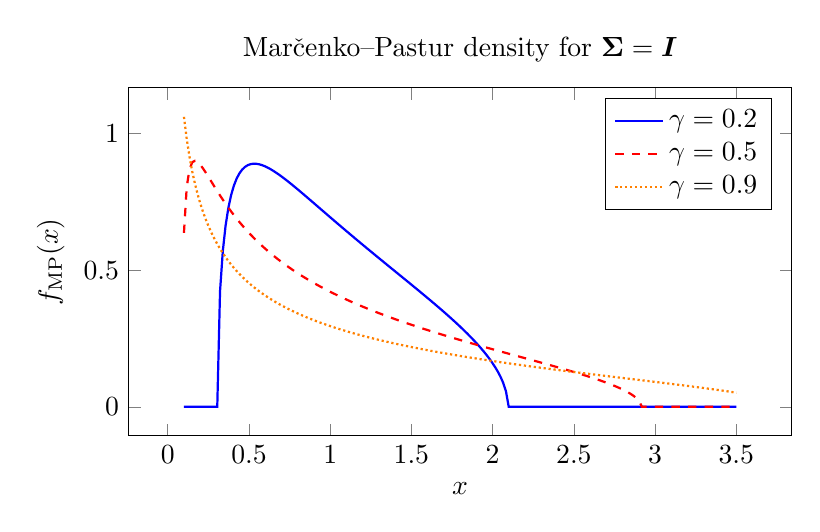
\begin{tikzpicture}
\begin{axis}[
  width=10cm, height=6cm,
  xlabel={$x$}, ylabel={$f_{\mathrm{MP}}(x)$},
  domain=0.1:3.5, samples=200,
  legend pos=north east,
  title={Mar\v{c}enko--Pastur density for $\bSigma=\bm{I}$}
]
% c = 0.2
\addplot[thick, blue] {(x >= (1-sqrt(0.2))^2 && x <= (1+sqrt(0.2))^2) * sqrt(((1+sqrt(0.2))^2 - x)*(x-(1-sqrt(0.2))^2))/(2*3.14159*0.2*x)};
\addlegendentry{$\gamma=0.2$}
% c = 0.5
\addplot[thick, red, dashed] {(x >= (1-sqrt(0.5))^2 && x <= (1+sqrt(0.5))^2) * sqrt(((1+sqrt(0.5))^2 - x)*(x-(1-sqrt(0.5))^2))/(2*3.14159*0.5*x)};
\addlegendentry{$\gamma=0.5$}
% c = 0.9
\addplot[thick, orange, densely dotted] {(x >= (1-sqrt(0.9))^2 && x <= (1+sqrt(0.9))^2) * sqrt(((1+sqrt(0.9))^2 - x)*(x-(1-sqrt(0.9))^2))/(2*3.14159*0.9*x)};
\addlegendentry{$\gamma=0.9$}
\end{axis}
\end{tikzpicture}
\caption{As $\gamma = p/T$ increases, eigenvalue dispersion grows, destabilizing inversion.}
\label{fig:mp-law}
\end{figure}

\subsection{Roadmap}

This document is organized as follows:
\begin{enumerate}[nosep]
  \item \textbf{Section~\ref{sec:background}}: Mathematical foundations---exponential families, conjugacy, graphical models.
  \item \textbf{Section~\ref{sec:horseshoe}}: The horseshoe prior and the graphical horseshoe model.
  \item \textbf{Section~\ref{sec:mcmc}}: MCMC methods---Gibbs sampling and NUTS.
  \item \textbf{Section~\ref{sec:vi}}: Variational inference---ADVI and its failure modes.
  \item \textbf{Section~\ref{sec:freq}}: Frequentist benchmarks---graphical lasso, Ledoit--Wolf.
  \item \textbf{Section~\ref{sec:evaluation}}: Evaluation metrics and experimental design.
  \item \textbf{Section~\ref{sec:portfolio}}: Downstream portfolio construction.
  \item \textbf{Section~\ref{sec:implementation}}: Full implementation guide with code.
  \item \textbf{Section~\ref{sec:extensions}}: Potential extensions and future directions.
\end{enumerate}

%======================================================================
\section{Mathematical Background}\label{sec:background}
%======================================================================

\subsection{The Multivariate Gaussian and Its Precision Matrix}

\begin{definition}[Multivariate Gaussian in Information Form]
The density of $\bm{y} \sim \Normal(\bm{\mu}, \bSigma)$ can equivalently be written in \emph{information form}:
\begin{equation}
  p(\bm{y} \mid \bOmega, \bm{\eta}) = \frac{|\bOmega|^{1/2}}{(2\pi)^{p/2}} \exp\!\Big(-\tfrac{1}{2}\bm{y}^\top \bOmega\,\bm{y} + \bm{\eta}^\top\bm{y} - A(\bm{\eta},\bOmega)\Big),
\end{equation}
where $\bm{\eta} = \bOmega\bm{\mu}$ is the \emph{natural parameter} (information vector) and $A(\cdot)$ is the log-partition function.
\end{definition}

For zero-mean data ($\bm{\mu}=\bm{0}$), the sufficient statistics are $\bm{S} = \sum_{k=1}^T \bm{y}_k\bm{y}_k^\top$ and the log-likelihood becomes:
\begin{equation}\label{eq:loglik}
  \ell(\bOmega) = \frac{T}{2}\log|\bOmega| - \frac{1}{2}\tr(\bm{S}\,\bOmega).
\end{equation}

\subsection{Exponential Families and Conjugacy}

The Gaussian likelihood in Eq.~\eqref{eq:loglik} is an exponential family in $\bOmega$, with natural parameter $\bOmega$ and sufficient statistic $\bm{S}$. Its conjugate prior is the \emph{Wishart distribution}.

\begin{definition}[Wishart Distribution]
$\bOmega \sim \Wishartd_p(\nu, \bm{V})$ has density
\begin{equation}
  p(\bOmega \mid \nu, \bm{V}) = \frac{|\bOmega|^{(\nu-p-1)/2}\exp(-\frac{1}{2}\tr(\bm{V}^{-1}\bOmega))}{2^{\nu p/2}|\bm{V}|^{\nu/2}\,\Gamma_p(\nu/2)},
  \quad \bOmega \in \Spp,
\end{equation}
where $\Gamma_p$ is the multivariate gamma function and $\nu > p-1$ degrees of freedom.
\end{definition}

\begin{proposition}[Conjugate Update]
With prior $\bOmega \sim \Wishartd_p(\nu_0, \bm{V}_0)$ and data $\bm{y}_1,\ldots,\bm{y}_T \stackrel{\text{iid}}{\sim}\Normal(\bm{0},\bOmega^{-1})$:
\begin{equation}
  \bOmega \mid \bm{y}_{1:T} \sim \Wishartd_p\!\left(\nu_0 + T,\; (\bm{V}_0^{-1} + \bm{S})^{-1}\right).
\end{equation}
\end{proposition}
\begin{proof}
Multiply the Wishart density by the likelihood in Eq.~\eqref{eq:loglik} and collect terms in $\bOmega$.
\end{proof}

\begin{keyinsight}
While the Wishart conjugate prior is convenient, it \emph{cannot encode sparsity}. It treats all off-diagonal elements symmetrically. The graphical horseshoe breaks this limitation by placing element-wise shrinkage priors on $\omega_{ij}$.
\end{keyinsight}

\subsection{Gaussian Graphical Models}

\begin{definition}[Gaussian Graphical Model]
An undirected graph $G = (V, E)$ with $|V| = p$ defines a GGM if $\bm{y} \sim \Normal(\bm{0}, \bOmega^{-1})$ and $\omega_{ij} = 0$ for all $(i,j) \notin E$. The graph encodes the conditional independence structure of $\bm{y}$.
\end{definition}

% ── Graphical model diagram ──
\begin{figure}[h]
\centering
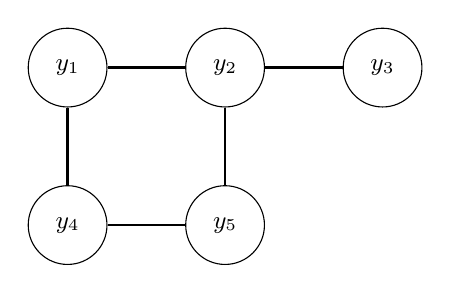
\begin{tikzpicture}[
  node distance=2cm,
  every node/.style={circle, draw, minimum size=1cm, font=\small}
]
\node (1) {$y_1$};
\node (2) [right of=1] {$y_2$};
\node (3) [right of=2] {$y_3$};
\node (4) [below of=1] {$y_4$};
\node (5) [below of=2] {$y_5$};

\draw[thick] (1) -- (2);
\draw[thick] (2) -- (3);
\draw[thick] (1) -- (4);
\draw[thick] (4) -- (5);
\draw[thick] (2) -- (5);

% Missing edges = conditional independence
\end{tikzpicture}
\caption{A 5-node GGM. Missing edges (e.g., $y_1$--$y_3$) correspond to zeros in $\bOmega$, i.e., conditional independence: $y_1 \perp y_3 \mid y_2, y_4, y_5$.}
\label{fig:ggm-example}
\end{figure}

\subsection{The Sparsity Assumption in Finance}

Under an approximate $K$-factor model, returns decompose as
\begin{equation}
  \bm{y}_t = \bm{B}\bm{f}_t + \bm{\epsilon}_t, \quad \bm{\epsilon}_t \sim \Normal(\bm{0},\bm{\Psi}),
\end{equation}
where $\bm{B}\in\R^{p\times K}$ is the loading matrix and $\bm{\Psi}$ is diagonal. The implied covariance is $\bSigma = \bm{B}\bm{B}^\top + \bm{\Psi}$. By the Woodbury identity,
\begin{equation}
  \bOmega = \bm{\Psi}^{-1} - \bm{\Psi}^{-1}\bm{B}(\bm{I}_K + \bm{B}^\top\bm{\Psi}^{-1}\bm{B})^{-1}\bm{B}^\top\bm{\Psi}^{-1}.
\end{equation}
If the residual precision $\bm{\Psi}^{-1}$ is diagonal and $K \ll p$, then $\bOmega$ is approximately sparse: most off-diagonal entries are near zero, with nonzero entries arising from direct stock-specific links not mediated by factors.

%======================================================================
\section{The Horseshoe Prior and Graphical Horseshoe}\label{sec:horseshoe}
%======================================================================

\subsection{The Original Horseshoe Prior}

Introduced by Carvalho, Polson, and Scott (2010) for sparse normal means estimation.

\begin{definition}[Horseshoe Prior]
For a signal vector $\bm{\theta} \in \R^p$:
\begin{equation}\label{eq:horseshoe}
  \theta_j \mid \lambda_j, \tau \sim \Normal(0, \lambda_j^2\tau^2), \quad
  \lambda_j \sim \HalfCauchy(0,1), \quad
  \tau \sim \HalfCauchy(0,1).
\end{equation}
\end{definition}

The half-Cauchy density is $p(\lambda) = \frac{2}{\pi(1+\lambda^2)}$ for $\lambda > 0$. Key properties:

\paragraph{Marginal prior on $\theta_j$.} Integrating out $\lambda_j$:
\begin{equation}
  p(\theta_j \mid \tau) = \int_0^\infty \Normal(\theta_j; 0, \lambda_j^2\tau^2)\;\frac{2}{\pi(1+\lambda_j^2)}\,d\lambda_j.
\end{equation}
This marginal has:
\begin{itemize}[nosep]
  \item An \emph{infinitely tall spike at zero} (like the Cauchy), encouraging shrinkage of noise.
  \item \emph{Polynomially heavy tails} ($\sim |\theta_j|^{-2}\log|\theta_j|$), allowing signals to escape.
\end{itemize}

\paragraph{Shrinkage coefficient.} Define $\kappa_j = \frac{1}{1 + \lambda_j^2\tau^2}$. The posterior mean under a Gaussian likelihood satisfies:
\begin{equation}
  \E[\theta_j \mid \bm{y}] \approx (1 - \E[\kappa_j \mid \bm{y}])\;\hat\theta_j^{\text{MLE}}.
\end{equation}
The horseshoe induces a \emph{bimodal} distribution on $\kappa_j$: values cluster near 0 (no shrinkage---signal) or near 1 (full shrinkage---noise).

% ── Horseshoe vs other priors visualization ──
\begin{figure}[h]
\centering
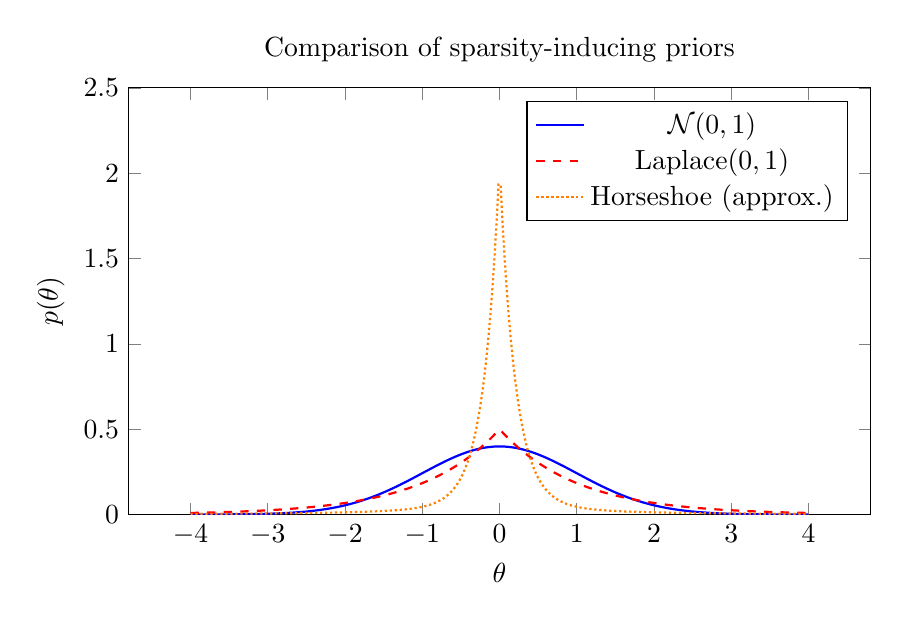
\begin{tikzpicture}
\begin{axis}[
  width=11cm, height=7cm,
  xlabel={$\theta$}, ylabel={$p(\theta)$},
  domain=-4:4, samples=300,
  ymin=0, ymax=2.5,
  legend pos=north east,
  title={Comparison of sparsity-inducing priors}
]
% Gaussian (sigma=1)
\addplot[thick, blue] {exp(-x^2/2)/sqrt(2*3.14159)};
\addlegendentry{$\Normal(0,1)$}
% Laplace (b=1)
\addplot[thick, red, dashed] {0.5*exp(-abs(x))};
\addlegendentry{Laplace$(0,1)$}
% Horseshoe (approximation: heavy spike + heavy tail)
\addplot[thick, orange, densely dotted] {0.8*2.5*exp(-abs(x)*5) + 0.2*1/(3.14159*(1+x^2))};
\addlegendentry{Horseshoe (approx.)}
\end{axis}
\end{tikzpicture}
\caption{The horseshoe combines a tall spike at zero (stronger than Laplace) with heavy tails (heavier than Gaussian), achieving aggressive shrinkage of noise while preserving signals.}
\label{fig:prior-comparison}
\end{figure}

\subsection{The Graphical Horseshoe (Li, Craig, Bhadra 2019)}

Apply the horseshoe element-wise to the off-diagonal entries of $\bOmega$:

\begin{definition}[Graphical Horseshoe Model]\label{def:graph-horseshoe}
Given observations $\bm{y}_1,\ldots,\bm{y}_T \stackrel{\text{iid}}{\sim}\Normal(\bm{0},\bOmega^{-1})$:
\begin{align}
  \bm{y}_k \mid \bOmega &\sim \Normal(\bm{0}, \bOmega^{-1}), \quad k=1,\ldots,T, \label{eq:gh-lik}\\
  \omega_{ij} \mid \lambda_{ij}, \tau &\sim \Normal(0, \lambda_{ij}^2\tau^2), \quad i < j, \label{eq:gh-offdiag}\\
  \lambda_{ij} &\sim \HalfCauchy(0,1), \quad i < j, \label{eq:gh-local}\\
  \tau &\sim \HalfCauchy(0,1), \label{eq:gh-global}\\
  \omega_{ii} &\propto 1, \quad \text{subject to } \bOmega \in \Spp. \label{eq:gh-diag}
\end{align}
\end{definition}

\begin{remark}
The positive-definiteness constraint $\bOmega \in \Spp$ is crucial and makes the model non-trivial. Each off-diagonal $\omega_{ij}$ cannot be updated independently; the constraint couples all elements.
\end{remark}

\paragraph{Parameter count.} The model has:
\begin{itemize}[nosep]
  \item $\binom{p}{2}$ off-diagonal precision entries $\omega_{ij}$,
  \item $\binom{p}{2}$ local shrinkage parameters $\lambda_{ij}$,
  \item $p$ diagonal entries $\omega_{ii}$,
  \item 1 global shrinkage parameter $\tau$.
\end{itemize}
Total: $p^2 + 1$ parameters (for symmetric $\bOmega$), growing quadratically in $p$.

\subsection{Why Horseshoe Over Alternatives?}

\begin{table}[h]
\centering
\caption{Comparison of priors for precision matrix estimation.}
\label{tab:prior-comparison}
\begin{tabular}{@{}lcccc@{}}
\toprule
\textbf{Prior/Method} & \textbf{Spike at 0} & \textbf{Heavy tails} & \textbf{Adaptive} & \textbf{Bayesian} \\
\midrule
Wishart/Inv-Wishart & \texttimes & \texttimes & \texttimes & \checkmark \\
LKJ prior & \texttimes & \texttimes & \texttimes & \checkmark \\
Bayesian Lasso & Moderate & \texttimes & \texttimes & \checkmark \\
Spike-and-slab & \checkmark & \checkmark & \checkmark & \checkmark \\
Horseshoe & \checkmark & \checkmark & \checkmark & \checkmark \\
Graphical Lasso & Point mass & \texttimes & \texttimes & \texttimes \\
\bottomrule
\end{tabular}
\end{table}

The spike-and-slab is the ``gold standard'' for variable selection but introduces $2^{p(p-1)/2}$ discrete configurations. The horseshoe is a \emph{continuous} relaxation that achieves nearly the same shrinkage profile without combinatorial model spaces.


%======================================================================
\section{MCMC: Gibbs Sampling and NUTS}\label{sec:mcmc}
%======================================================================

\subsection{Gibbs Sampler (Li et al., 2019)}

Li et al.\ develop a block Gibbs sampler by exploiting the column-wise structure of $\bOmega$. The key idea: partition $\bOmega$ into column $j$ and the rest, then update column $j$ conditional on all others.

\paragraph{Column-wise decomposition.} Partition:
\begin{equation}
  \bOmega = \begin{pmatrix} \bOmega_{-j,-j} & \bm{\omega}_{-j,j} \\ \bm{\omega}_{-j,j}^\top & \omega_{jj} \end{pmatrix}, \quad
  \bm{S} = \begin{pmatrix} \bm{S}_{-j,-j} & \bm{s}_{-j,j} \\ \bm{s}_{-j,j}^\top & s_{jj} \end{pmatrix}.
\end{equation}

The conditional distribution of $(\bm{\omega}_{-j,j}, \omega_{jj})$ given the rest and the horseshoe hyperparameters can be derived in closed form:
\begin{align}
  \bm{\omega}_{-j,j} \mid \omega_{jj}, \bm{\Lambda}_j, \tau, \bm{S}
  &\sim \Normal\!\left(-\frac{\bm{C}_j\,\bm{s}_{-j,j}}{s_{jj}},\;\frac{\bm{C}_j}{s_{jj} + T}\right) \text{ truncated to } \bOmega \succ 0,\\
  \omega_{jj} \mid \bm{\omega}_{-j,j}, \bm{S}
  &\sim \text{Gamma}\!\left(\frac{T}{2}+1,\;\frac{s_{jj}}{2}\right) + \bm{\omega}_{-j,j}^\top\bOmega_{-j,-j}^{-1}\bm{\omega}_{-j,j},
\end{align}
where $\bm{C}_j = \big(s_{jj}\,\bOmega_{-j,-j} + \text{diag}(\lambda_{1j}^{-2}\tau^{-2},\ldots)^{-1}\big)^{-1}$ and $\bm{\Lambda}_j$ collects local parameters for column $j$.

\paragraph{Updating local/global shrinkage.} The half-Cauchy priors are handled via the data-augmentation trick:
\begin{equation}
  \lambda_{ij}^2 \mid \omega_{ij}, \tau, \nu_{ij} \sim \text{InvGamma}\!\left(1, \frac{1}{\nu_{ij}} + \frac{\omega_{ij}^2}{2\tau^2}\right), \quad
  \nu_{ij} \sim \text{InvGamma}\!\left(1, 1 + \frac{1}{\lambda_{ij}^2}\right).
\end{equation}
Similarly for $\tau^2$ and its auxiliary $\xi$.

\begin{algorithm}
\caption{Graphical Horseshoe Gibbs Sampler (one sweep)}
\label{alg:gibbs}
\begin{algorithmic}[1]
\For{$j = 1, \ldots, p$}
  \State Compute $\bm{C}_j$ using current $\bOmega_{-j,-j}$, $\bm{\Lambda}_j$, $\tau$
  \State Sample $\bm{\omega}_{-j,j}$ from truncated Normal
  \State Sample $\omega_{jj}$ from shifted Gamma
\EndFor
\For{$i < j$}
  \State Sample $\nu_{ij} \sim \text{InvGamma}(1, 1+1/\lambda_{ij}^2)$
  \State Sample $\lambda_{ij}^2 \sim \text{InvGamma}(1, 1/\nu_{ij} + \omega_{ij}^2/(2\tau^2))$
\EndFor
\State Sample $\xi \sim \text{InvGamma}(1, 1 + 1/\tau^2)$
\State Sample $\tau^2 \sim \text{InvGamma}\!\big(\frac{p(p-1)/2+1}{2},\; \frac{1}{\xi} + \frac{1}{2}\sum_{i<j}\omega_{ij}^2/\lambda_{ij}^2\big)$
\end{algorithmic}
\end{algorithm}

\paragraph{Computational cost.} Each sweep requires $p$ solves of $(p{-}1)\times(p{-}1)$ linear systems: $O(p^3)$ per sweep, $O(Np^3)$ for $N$ iterations total.

\subsection{Hamiltonian Monte Carlo and NUTS}

\subsubsection{HMC Fundamentals}

Hamiltonian Monte Carlo augments the target $\pi(\bm{\theta})$ with auxiliary momentum $\bm{r} \sim \Normal(\bm{0},\bm{M})$:
\begin{equation}
  H(\bm{\theta},\bm{r}) = -\log\pi(\bm{\theta}) + \tfrac{1}{2}\bm{r}^\top\bm{M}^{-1}\bm{r}.
\end{equation}
Hamilton's equations define a trajectory:
\begin{align}
  \frac{d\bm{\theta}}{dt} &= \bm{M}^{-1}\bm{r}, &
  \frac{d\bm{r}}{dt} &= \nabla_{\bm{\theta}}\log\pi(\bm{\theta}).
\end{align}

The \emph{leapfrog integrator} with step size $\epsilon$ and $L$ steps approximates this trajectory:
\begin{align}
  \bm{r}_{t+\epsilon/2} &= \bm{r}_t + \frac{\epsilon}{2}\nabla_{\bm{\theta}}\log\pi(\bm{\theta}_t), \\
  \bm{\theta}_{t+\epsilon} &= \bm{\theta}_t + \epsilon\,\bm{M}^{-1}\bm{r}_{t+\epsilon/2}, \\
  \bm{r}_{t+\epsilon} &= \bm{r}_{t+\epsilon/2} + \frac{\epsilon}{2}\nabla_{\bm{\theta}}\log\pi(\bm{\theta}_{t+\epsilon}).
\end{align}

\subsubsection{The No-U-Turn Sampler (NUTS)}

NUTS (Hoffman and Gelman, 2014) eliminates the need to tune $L$ by building a balanced binary tree of leapfrog steps, doubling the trajectory until a ``U-turn'' criterion is met:
\begin{equation}
  (\bm{\theta}^+ - \bm{\theta}^-)\cdot\bm{r}^- < 0 \quad \text{or} \quad (\bm{\theta}^+ - \bm{\theta}^-)\cdot\bm{r}^+ < 0,
\end{equation}
where $\bm{\theta}^{\pm}$ are the endpoints and $\bm{r}^{\pm}$ their momenta.

\begin{keyinsight}
NUTS requires gradients of the log-posterior. For the graphical horseshoe, this means differentiating through the positive-definiteness constraint. NumPyro handles this via a Cholesky reparameterization: $\bOmega = \bm{L}\bm{L}^\top$ where $\bm{L}$ is lower-triangular with positive diagonal, mapped to unconstrained space via $\log$ on diagonal elements.
\end{keyinsight}

\paragraph{Advantages of NUTS over Gibbs for this model:}
\begin{enumerate}[nosep]
  \item Joint updates of all parameters (vs.\ column-by-column Gibbs): better mixing in correlated posteriors.
  \item Automatic trajectory length adaptation.
  \item JAX/GPU acceleration via NumPyro.
\end{enumerate}

\paragraph{Disadvantages:}
\begin{enumerate}[nosep]
  \item Gradient cost per leapfrog step is $O(p^3)$ (Cholesky + log-det differentiation).
  \item Heavy-tailed half-Cauchy creates challenging geometry (funnels).
  \item Memory scales with trajectory tree depth.
\end{enumerate}

\subsection{Diagnosing MCMC Convergence}

\paragraph{$\hat{R}$ (Gelman--Rubin diagnostic).} Run $M$ chains of length $N$. Compute between-chain ($B$) and within-chain ($W$) variances:
\begin{equation}
  \hat{R} = \sqrt{\frac{(N-1)/N \cdot W + B/N}{W}}.
\end{equation}
Values $\hat{R} > 1.01$ indicate non-convergence (Vehtari et al., 2021).

\paragraph{Effective Sample Size (ESS).} Accounts for autocorrelation:
\begin{equation}
  \text{ESS} = \frac{MN}{1 + 2\sum_{k=1}^{\infty}\rho_k},
\end{equation}
where $\rho_k$ is the lag-$k$ autocorrelation. Bulk ESS $> 400$ per chain is recommended.

\paragraph{Divergent transitions.} In NUTS, a divergence occurs when the leapfrog integrator's Hamiltonian error exceeds a threshold. Divergences indicate regions of high curvature that the sampler cannot navigate, common with half-Cauchy priors (the ``funnel'' problem).

\begin{warning}
The horseshoe posterior often exhibits a \emph{Neal's funnel} geometry: when $\lambda_{ij}$ is near zero, $\omega_{ij}$ is tightly concentrated, creating extreme curvature. Reparameterization (non-centered parameterization) is essential. In NumPyro, use:
\begin{lstlisting}
omega_raw = numpyro.sample("omega_raw", dist.Normal(0, 1))
omega_ij = omega_raw * lambda_ij * tau  # non-centered
\end{lstlisting}
\end{warning}


%======================================================================
\section{Variational Inference}\label{sec:vi}
%======================================================================

\subsection{The Variational Objective}

Variational inference approximates the intractable posterior $p(\bm{\theta}\mid\bm{y})$ by the closest member of a tractable family $\mathcal{Q}$:
\begin{equation}
  q^*(\bm{\theta}) = \arg\min_{q \in \mathcal{Q}} \KL\big(q(\bm{\theta})\;\|\;p(\bm{\theta}\mid\bm{y})\big).
\end{equation}

Equivalently, maximize the \emph{Evidence Lower Bound} (ELBO):
\begin{equation}\label{eq:elbo}
  \ELBO(q) = \E_q[\log p(\bm{y},\bm{\theta})] - \E_q[\log q(\bm{\theta})] = \log p(\bm{y}) - \KL(q\|p(\cdot\mid\bm{y})) \leq \log p(\bm{y}).
\end{equation}

\begin{keyinsight}
The gap between the ELBO and the log-evidence is exactly $\KL(q\|p)$. Since KL divergence is non-negative and equals zero iff $q = p$ a.e., maximizing the ELBO is equivalent to minimizing the KL divergence. But the KL is \emph{asymmetric}: $\KL(q\|p)$ penalizes $q$ for placing mass where $p$ is small (mode-seeking), leading to underestimation of posterior variance.
\end{keyinsight}

\subsection{Mean-Field Approximation}

The mean-field family assumes full posterior independence:
\begin{equation}
  q(\bm{\theta}) = \prod_{d=1}^{D} q_d(\theta_d).
\end{equation}
For the graphical horseshoe with parameters $\bm{\theta} = (\bOmega, \blambda, \tau)$, this means:
\begin{equation}
  q(\bOmega, \blambda, \tau) = \left(\prod_{i \leq j} q_{ij}(\omega_{ij})\right)\left(\prod_{i<j}q_{ij}^{\lambda}(\lambda_{ij})\right)q^{\tau}(\tau).
\end{equation}

\begin{warning}
Mean-field VI \textbf{assumes posterior independence between $\omega_{ij}$ and $\lambda_{ij}$}. But the horseshoe's power comes from the strong posterior dependence between these: when $\lambda_{ij}$ is small, $\omega_{ij}$ should be near zero; when $\lambda_{ij}$ is large, $\omega_{ij}$ should be close to its MLE. Breaking this coupling may destroy the bimodal shrinkage profile.
\end{warning}

\subsection{Automatic Differentiation Variational Inference (ADVI)}

ADVI (Kucukelbir et al., 2017) automates VI for any differentiable probability model:

\begin{enumerate}
  \item \textbf{Transform} all constrained parameters to $\R^D$ via bijections $T$:
  \begin{equation}
    \bm{\zeta} = T(\bm{\theta}), \quad \text{e.g., } \zeta_{ij} = \log(\lambda_{ij})\text{ for }\lambda_{ij} > 0.
  \end{equation}
  For the precision matrix constraint $\bOmega \succ 0$, use the Cholesky factor with log-diagonal.

  \item \textbf{Approximate} in the unconstrained space with a Gaussian:
  \begin{align}
    \text{Mean-field:} &\quad q(\bm{\zeta}) = \prod_d \Normal(\zeta_d; \mu_d, \sigma_d^2), \\
    \text{Full-rank:} &\quad q(\bm{\zeta}) = \Normal(\bm{\zeta}; \bm{\mu}, \bm{L}\bm{L}^\top).
  \end{align}

  \item \textbf{Optimize} via stochastic gradient ascent on the ELBO, using the reparameterization trick:
  \begin{equation}
    \bm{\zeta} = \bm{\mu} + \bm{L}\bm{\epsilon}, \quad \bm{\epsilon} \sim \Normal(\bm{0},\bm{I}),
  \end{equation}
  so that $\nabla_{\bm{\mu},\bm{L}}\ELBO = \E_{\bm{\epsilon}}[\nabla_{\bm{\mu},\bm{L}}\log p(\bm{y},T^{-1}(\bm{\mu}+\bm{L}\bm{\epsilon})) + \text{entropy terms}]$.
\end{enumerate}

\paragraph{ADVI parameter count.}
\begin{itemize}[nosep]
  \item Mean-field: $2D$ parameters ($\mu_d, \log\sigma_d$ for each dimension).
  \item Full-rank: $D + D(D+1)/2$ parameters (mean + lower-triangular Cholesky factor).
\end{itemize}
For $p=50$: $D \approx 50\cdot51/2 + 50\cdot49/2 + 50\cdot49/2 + 1 \approx 3726$. Full-rank ADVI would optimize $\sim 7$ million parameters---likely infeasible.

\subsection{Expected Failure Modes for the Horseshoe}

\subsubsection{Loss of Bimodal Shrinkage}

The horseshoe posterior on $\kappa_j = 1/(1+\lambda_j^2\tau^2)$ is typically bimodal: mass near 0 and near 1. A Gaussian $q(\log\lambda_{ij})$ is unimodal in $\lambda_{ij}$-space, so $q(\kappa_j)$ is also unimodal. This means:

\begin{itemize}[nosep]
  \item VI cannot represent the ``shrink or don't'' behavior.
  \item It will compromise: moderate shrinkage on \emph{all} entries.
  \item Result: signals are over-shrunk, noise is under-shrunk.
\end{itemize}

\subsubsection{Underestimation of Posterior Uncertainty}

Since $\KL(q\|p)$ is mode-seeking:
\begin{equation}
  \Var_q[\omega_{ij}] \leq \Var_{p(\cdot|\bm{y})}[\omega_{ij}] \quad \text{(typically)}.
\end{equation}
This means VI-based credible intervals will be too narrow, potentially affecting downstream portfolio decisions.

\subsubsection{Sensitivity to Initialization}

The ELBO landscape for heavy-tailed priors is often multimodal. Different random seeds may converge to different local optima, with $\tau$ collapsing to near-zero (over-shrinkage) or exploding (no shrinkage).


%======================================================================
\section{Frequentist Benchmarks}\label{sec:freq}
%======================================================================

\subsection{The Graphical Lasso}

The graphical lasso (Friedman et al., 2008) solves the $\ell_1$-penalized log-likelihood:
\begin{equation}\label{eq:glasso}
  \hat\bOmega_{\text{glasso}} = \arg\max_{\bOmega \succ 0} \left\{ \log|\bOmega| - \tr(\hat\bSigma\,\bOmega) - \rho\sum_{i\neq j}|\omega_{ij}| \right\},
\end{equation}
where $\rho > 0$ is the penalty parameter. This is a convex program solved by coordinate descent.

\begin{remark}
The graphical lasso is the MAP estimator under a Bayesian model with independent Laplace (double-exponential) priors on off-diagonal entries. The horseshoe dominates the Laplace for sparse estimation because the Laplace has exponential tails (too light for large signals) and a non-differentiable but finite spike at zero (not aggressive enough for noise).
\end{remark}

\subsection{Ledoit--Wolf Linear Shrinkage}

The linear shrinkage estimator:
\begin{equation}
  \hat\bSigma_{\text{LW}} = \alpha\,\hat\bSigma + (1-\alpha)\,\bm{F},
\end{equation}
where $\bm{F}$ is a structured target (e.g., $\mu\bm{I}$ or the single-factor model covariance) and $\alpha^*$ minimizes the expected Frobenius loss. Ledoit and Wolf (2004) provide an analytical formula for $\alpha^*$.

\subsection{The Sample Covariance (Baseline)}

Included as a baseline. Recall that for $p/T > 1$, $\hat\bSigma$ is singular and $\hat\bOmega$ does not exist.

\subsection{Summary of Benchmarks}

\begin{table}[h]
\centering
\caption{Frequentist estimators in our comparison.}
\begin{tabular}{@{}lccc@{}}
\toprule
\textbf{Method} & \textbf{Sparsity} & \textbf{Tuning} & \textbf{Works for $p > T$?} \\
\midrule
Sample covariance & No & None & No \\
Ledoit--Wolf & No & Analytical $\alpha$ & Yes \\
Graphical lasso & Yes & $\rho$ (CV) & Yes \\
\bottomrule
\end{tabular}
\end{table}


%======================================================================
\section{Evaluation Metrics}\label{sec:evaluation}
%======================================================================

\subsection{Loss Functions for Precision Matrices}

\paragraph{Stein's loss (entropy loss).}
\begin{equation}
  L_S(\hat\bOmega, \bOmega_0) = \tr(\hat\bOmega^{-1}\bOmega_0) - \log|\hat\bOmega^{-1}\bOmega_0| - p.
\end{equation}
This is the KL divergence $\KL(\Normal(0,\hat\bOmega^{-1})\|\Normal(0,\bOmega_0^{-1}))$. It is zero iff $\hat\bOmega = \bOmega_0$.

\paragraph{Frobenius loss.}
\begin{equation}
  L_F(\hat\bOmega, \bOmega_0) = \|\hat\bOmega - \bOmega_0\|_F^2 = \sum_{i,j}(\hat\omega_{ij} - \omega_{ij}^{(0)})^2.
\end{equation}

\paragraph{Spectral norm loss.}
\begin{equation}
  L_2(\hat\bOmega, \bOmega_0) = \|\hat\bOmega - \bOmega_0\|_2 = \sigma_{\max}(\hat\bOmega - \bOmega_0).
\end{equation}

\subsection{Sparsity Recovery Metrics}

Treating $\omega_{ij} = 0$ as ``no edge'' and $\omega_{ij}\neq 0$ as ``edge'':
\begin{itemize}[nosep]
  \item \textbf{True Positive Rate (TPR/Recall):} $\frac{\text{TP}}{\text{TP}+\text{FN}}$---fraction of true edges recovered.
  \item \textbf{False Positive Rate (FPR):} $\frac{\text{FP}}{\text{FP}+\text{TN}}$---fraction of non-edges falsely declared edges.
  \item \textbf{Matthews Correlation Coefficient (MCC):} Balanced metric, $\in[-1,1]$.
  \item \textbf{F1 score}: Harmonic mean of precision and recall.
\end{itemize}

For the horseshoe, edge detection uses a credible interval criterion: edge $(i,j)$ is declared present if the 95\% posterior interval for $\omega_{ij}$ excludes zero.

\subsection{Eigenvalue Spectrum Comparison}

Compare eigenvalue distributions of $\hat\bOmega$ against $\bOmega_0$ (for synthetic data) or the oracle estimator.

\subsection{Experimental Design Matrix}

\begin{table}[h]
\centering
\caption{Full experimental grid.}
\label{tab:experiment-grid}
\begin{tabular}{@{}ll@{}}
\toprule
\textbf{Factor} & \textbf{Levels} \\
\midrule
Dimension $p$ & 50, 100 \\
Sample size $T$ & 75, 120, 250, 500 \\
Methods & Sample Cov, Ledoit--Wolf, Glasso, NUTS, ADVI-MF, ADVI-FR \\
Data source & Synthetic (known $\bOmega_0$), CRSP equity returns \\
\midrule
Total experiments & $2 \times 4 \times 6 \times 2 = 96$ configurations \\
\bottomrule
\end{tabular}
\end{table}


%======================================================================
\section{Downstream Application: Portfolio Construction}\label{sec:portfolio}
%======================================================================

\subsection{Global Minimum Variance Portfolio}

Given an estimate $\hat\bOmega$, the GMV portfolio weights are:
\begin{equation}
  \bm{w}^* = \frac{\hat\bOmega\,\bm{1}}{\bm{1}^\top\hat\bOmega\,\bm{1}}.
\end{equation}
Note: this requires only $\hat\bOmega$, not $\hat\bSigma$.

\subsection{Out-of-Sample Evaluation}

For each rolling window of length $T$:
\begin{enumerate}[nosep]
  \item Estimate $\hat\bOmega$ from data in $[t-T, t)$.
  \item Compute weights $\bm{w}^*_t$.
  \item Evaluate out-of-sample portfolio variance: $\sigma^2_{\text{oos},t} = (\bm{w}^*_t)^\top\hat\bSigma_{\text{future}}(\bm{w}^*_t)$, where $\hat\bSigma_{\text{future}}$ is estimated from $[t, t+T)$.
\end{enumerate}

\subsection{Bayesian Portfolio Uncertainty}

With MCMC, we obtain posterior samples $\bOmega^{(1)},\ldots,\bOmega^{(N)}$, yielding weight samples $\bm{w}^{(1)},\ldots,\bm{w}^{(N)}$. This gives a full posterior distribution over portfolio weights---a major advantage of the Bayesian approach.

\begin{equation}
  \text{Posterior predictive volatility:} \quad \sigma_{\text{pred}} = \sqrt{\frac{1}{N}\sum_{n=1}^N (\bm{w}^{(n)})^\top\hat\bSigma_{\text{oos}}\,\bm{w}^{(n)}}.
\end{equation}


%======================================================================
\section{Implementation Guide}\label{sec:implementation}
%======================================================================

\subsection{Data Pipeline}

\begin{lstlisting}[caption={Loading and preprocessing CRSP data.}]
import pandas as pd
import numpy as np

# Load CRSP daily returns (assumed pre-downloaded from WRDS)
df = pd.read_csv("crsp_daily.csv", parse_dates=["date"])

# Select p most liquid large-cap stocks
top_stocks = (df.groupby("permno")["vol_usd"]
              .mean()
              .nlargest(100)
              .index)
returns = (df[df["permno"].isin(top_stocks)]
           .pivot(index="date", columns="permno", values="ret")
           .dropna())

# Demean and standardize
returns = (returns - returns.mean()) / returns.std()

# Create estimation windows
def get_window(returns, end_date, T):
    mask = returns.index <= end_date
    return returns[mask].tail(T).values  # (T, p) array
\end{lstlisting}

\subsection{NumPyro Model Specification}

\begin{lstlisting}[caption={Graphical horseshoe model in NumPyro.}]
import jax.numpy as jnp
import numpyro
import numpyro.distributions as dist
from numpyro.distributions import constraints

def graphical_horseshoe(Y, p):
    T = Y.shape[0]

    # Global shrinkage
    tau = numpyro.sample("tau", dist.HalfCauchy(1.0))

    # Local shrinkage (off-diagonal, upper triangle)
    n_offdiag = p * (p - 1) // 2
    lambdas = numpyro.sample("lambdas",
        dist.HalfCauchy(jnp.ones(n_offdiag)))

    # Off-diagonal entries (non-centered parameterization)
    omega_offdiag_raw = numpyro.sample("omega_offdiag_raw",
        dist.Normal(jnp.zeros(n_offdiag), 1.0))
    omega_offdiag = omega_offdiag_raw * lambdas * tau

    # Diagonal entries (must be positive)
    omega_diag = numpyro.sample("omega_diag",
        dist.HalfNormal(jnp.ones(p) * 5.0))

    # Assemble precision matrix
    Omega = jnp.zeros((p, p))
    triu_idx = jnp.triu_indices(p, k=1)
    Omega = Omega.at[triu_idx].set(omega_offdiag)
    Omega = Omega + Omega.T
    Omega = Omega + jnp.diag(omega_diag)

    # Likelihood (with positive-definiteness check)
    numpyro.sample("Y", dist.MultivariateNormal(
        loc=jnp.zeros(p),
        precision_matrix=Omega), obs=Y)
\end{lstlisting}

\begin{warning}
The above is a simplified version. In practice, you need to handle the positive-definiteness constraint carefully. NumPyro's \texttt{MultivariateNormal} with \texttt{precision\_matrix} internally computes the Cholesky decomposition, which will fail if $\bOmega \not\succ 0$. Strategies:
\begin{enumerate}[nosep]
  \item Use \texttt{LKJCholesky} as a base and add horseshoe perturbations.
  \item Reparameterize via the Cholesky factor directly.
  \item Use a potential function with a barrier for the PD constraint.
\end{enumerate}
\end{warning}

\subsection{Running NUTS}

\begin{lstlisting}[caption={Running NUTS inference.}]
from numpyro.infer import MCMC, NUTS
import jax

kernel = NUTS(graphical_horseshoe,
              target_accept_prob=0.85,
              max_tree_depth=10)

mcmc = MCMC(kernel,
            num_warmup=2000,
            num_samples=5000,
            num_chains=4)

mcmc.run(jax.random.PRNGKey(0), Y=Y_train, p=p)
mcmc.print_summary()

# Extract posterior samples
samples = mcmc.get_samples()
omega_samples = reconstruct_omega(samples)  # shape: (5000, p, p)
omega_hat_nuts = omega_samples.mean(axis=0)
\end{lstlisting}

\subsection{Running ADVI}

\begin{lstlisting}[caption={Running ADVI inference.}]
from numpyro.infer import SVI, Trace_ELBO
from numpyro.infer.autoguide import AutoNormal, AutoMultivariateNormal

# Mean-field ADVI
guide_mf = AutoNormal(graphical_horseshoe)
svi_mf = SVI(graphical_horseshoe, guide_mf,
             numpyro.optim.Adam(0.01), Trace_ELBO())

svi_result_mf = svi_mf.run(jax.random.PRNGKey(1),
                            num_steps=50000,
                            Y=Y_train, p=p)

# Full-rank ADVI
guide_fr = AutoMultivariateNormal(graphical_horseshoe)
svi_fr = SVI(graphical_horseshoe, guide_fr,
             numpyro.optim.Adam(0.005), Trace_ELBO())

svi_result_fr = svi_fr.run(jax.random.PRNGKey(2),
                            num_steps=100000,
                            Y=Y_train, p=p)

# Draw samples from the variational posterior
predictive = numpyro.infer.Predictive(guide_mf,
    params=svi_result_mf.params, num_samples=5000)
vi_samples = predictive(jax.random.PRNGKey(3),
                         Y=Y_train, p=p)
\end{lstlisting}

\subsection{Graphical Lasso Benchmark}

\begin{lstlisting}[caption={Graphical lasso via scikit-learn.}]
from sklearn.covariance import GraphicalLassoCV

glasso = GraphicalLassoCV(cv=5, max_iter=500)
glasso.fit(Y_train)

omega_hat_glasso = glasso.precision_
alpha_selected = glasso.alpha_
\end{lstlisting}

\subsection{Ledoit--Wolf Benchmark}

\begin{lstlisting}[caption={Ledoit--Wolf shrinkage estimator.}]
from sklearn.covariance import LedoitWolf

lw = LedoitWolf()
lw.fit(Y_train)

sigma_hat_lw = lw.covariance_
omega_hat_lw = np.linalg.inv(sigma_hat_lw)
shrinkage_intensity = lw.shrinkage_
\end{lstlisting}

\subsection{Synthetic Data Generation}

\begin{lstlisting}[caption={Generating data with known sparse precision matrix.}]
def generate_sparse_precision(p, sparsity=0.1, seed=42):
    """Generate a sparse PD precision matrix."""
    rng = np.random.default_rng(seed)

    # Start with identity
    Omega = np.eye(p)

    # Add random sparse off-diagonal entries
    n_edges = int(sparsity * p * (p - 1) / 2)
    triu_i, triu_j = np.triu_indices(p, k=1)
    selected = rng.choice(len(triu_i), n_edges, replace=False)

    for idx in selected:
        i, j = triu_i[idx], triu_j[idx]
        val = rng.choice([-1, 1]) * rng.uniform(0.3, 0.8)
        Omega[i, j] = val
        Omega[j, i] = val

    # Ensure positive definiteness via diagonal loading
    min_eig = np.linalg.eigvalsh(Omega).min()
    if min_eig < 0.1:
        Omega += (0.1 - min_eig) * np.eye(p)

    return Omega

def generate_data(Omega, T, seed=0):
    """Sample from N(0, Omega^{-1})."""
    Sigma = np.linalg.inv(Omega)
    return np.random.default_rng(seed).multivariate_normal(
        np.zeros(Omega.shape[0]), Sigma, size=T)
\end{lstlisting}

\subsection{Evaluation Code}

\begin{lstlisting}[caption={Computing loss metrics.}]
def steins_loss(Omega_hat, Omega_true):
    """Stein's loss = tr(Ohat^{-1} O) - log|Ohat^{-1} O| - p"""
    p = Omega_true.shape[0]
    Sigma_hat = np.linalg.inv(Omega_hat)
    M = Sigma_hat @ Omega_true
    return np.trace(M) - np.linalg.slogdet(M)[1] - p

def frobenius_loss(Omega_hat, Omega_true):
    return np.linalg.norm(Omega_hat - Omega_true, 'fro')**2

def sparsity_metrics(Omega_hat, Omega_true, threshold=1e-5):
    """TPR, FPR, MCC for edge recovery."""
    true_edges = np.abs(Omega_true) > threshold
    pred_edges = np.abs(Omega_hat) > threshold
    # Mask diagonal
    mask = ~np.eye(Omega_true.shape[0], dtype=bool)
    true_e = true_edges[mask]
    pred_e = pred_edges[mask]

    tp = (true_e & pred_e).sum()
    fp = (~true_e & pred_e).sum()
    fn = (true_e & ~pred_e).sum()
    tn = (~true_e & ~pred_e).sum()

    tpr = tp / max(tp + fn, 1)
    fpr = fp / max(fp + tn, 1)
    mcc_num = tp*tn - fp*fn
    mcc_den = np.sqrt((tp+fp)*(tp+fn)*(tn+fp)*(tn+fn))
    mcc = mcc_num / max(mcc_den, 1e-10)
    return {"TPR": tpr, "FPR": fpr, "MCC": mcc}
\end{lstlisting}


%======================================================================
\section{Potential Extensions and Future Directions}\label{sec:extensions}
%======================================================================

\subsection{Structured Variational Families}

Mean-field is the worst-case for the horseshoe. Richer families could preserve more of the shrinkage structure:

\begin{enumerate}
  \item \textbf{Normalizing flows}: Transform a simple base distribution through invertible maps to capture multimodality. The density is:
  \begin{equation}
    q(\bm{\theta}) = q_0(f^{-1}(\bm{\theta}))\left|\det\frac{\partial f^{-1}}{\partial\bm{\theta}}\right|.
  \end{equation}
  Candidates: RealNVP, Masked Autoregressive Flows (MAF), Neural Spline Flows.

  \item \textbf{Mixture variational families}: $q(\bm{\theta}) = \sum_{k=1}^K \pi_k \Normal(\bm{\mu}_k, \bm{\Sigma}_k)$. With $K=2$, this could represent the bimodal shrinkage profile.

  \item \textbf{Structured mean-field}: Group $(\omega_{ij}, \lambda_{ij})$ into blocks and allow within-block dependence:
  \begin{equation}
    q(\bm{\theta}) = q(\tau)\prod_{i<j}q_{ij}(\omega_{ij}, \lambda_{ij}).
  \end{equation}
\end{enumerate}

\subsection{Alternative MCMC Strategies}

\begin{enumerate}
  \item \textbf{Riemannian HMC}: Exploit the geometry of the positive-definite cone with a Fisher information metric. Higher per-step cost, but potentially much faster mixing.
  \item \textbf{Slice sampling within Gibbs}: For the half-Cauchy parameters, slice sampling avoids the auxiliary variable trick and may mix better.
  \item \textbf{Parallel tempering}: Run multiple chains at different temperatures to overcome multimodality.
\end{enumerate}

\subsection{Dynamic / Time-Varying Precision Matrices}

Equity return structure is non-stationary. Extensions:
\begin{enumerate}
  \item \textbf{DCC-type dynamics}: Allow $\bOmega_t$ to evolve via exponentially weighted past data.
  \item \textbf{State-space horseshoe}: $\bOmega_t = \bOmega_{t-1} + \bm{\Delta}_t$ with horseshoe priors on $\bm{\Delta}_t$ to encode \emph{sparsity of changes}.
  \item \textbf{Regime-switching}: Finite mixture of precision matrices, with HMM-type transitions between regimes (e.g., crisis vs.\ calm).
\end{enumerate}

\subsection{Non-Gaussian Likelihoods}

Stock returns are heavy-tailed. Replacements for the Gaussian likelihood:
\begin{enumerate}
  \item \textbf{Multivariate $t$-distribution}: $\bm{y}_k \sim t_\nu(\bm{0}, \bOmega^{-1})$. Introduces one additional parameter $\nu$ (degrees of freedom). The graphical model interpretation remains valid.
  \item \textbf{Copula models}: Separate marginal distributions (e.g., skewed $t$) from the dependence structure encoded in $\bOmega$ via a Gaussian copula.
  \item \textbf{Score-driven models (GAS)}: Update $\bOmega_t$ using the score of a heavy-tailed observation density.
\end{enumerate}

\subsection{Theoretical Analysis}

\begin{enumerate}
  \item \textbf{Posterior contraction rates}: Under what conditions on $(p, T, s)$ (where $s$ is the true sparsity) does the horseshoe posterior contract at the minimax rate? Existing results (e.g., van der Pas et al., 2014) are for the normal means problem; extending to the precision matrix setting is open.
  \item \textbf{VI approximation error bounds}: Characterize the gap $\|\hat\bOmega_{\text{VI}} - \hat\bOmega_{\text{MCMC}}\|$ as a function of $p/T$, the variational family, and the prior structure.
  \item \textbf{Decision-theoretic comparison}: Under Stein's loss, is there a formal dominance result for the horseshoe over the graphical lasso as $p/T \to \infty$?
\end{enumerate}


%======================================================================
\section{Visualization Plan}\label{sec:viz-plan}
%======================================================================

To communicate results effectively, we propose the following plots:

\begin{enumerate}
  \item \textbf{Heatmaps} of $\hat\bOmega$ across methods, side by side, for a fixed $(p,T)$.
  \item \textbf{Shrinkage profile plots}: Empirical distribution of $|\hat\omega_{ij}|$ for NUTS vs.\ ADVI, showing whether VI preserves the bimodal ``shrink or don't'' structure.
  \item \textbf{Loss vs.\ $p/T$ curves}: Stein's loss and Frobenius loss as $p/T$ varies, with error bars from multiple random seeds or rolling windows.
  \item \textbf{ROC curves} for sparsity recovery (synthetic data with known $\bOmega_0$).
  \item \textbf{Eigenvalue spectrum plots}: Comparing eigenvalues of $\hat\bOmega$ across methods against truth.
  \item \textbf{ELBO traces}: Convergence diagnostics for ADVI (mean-field vs.\ full-rank).
  \item \textbf{Trace plots and $\hat{R}$ summaries}: For NUTS chains.
  \item \textbf{Out-of-sample portfolio volatility} over rolling windows.
  \item \textbf{Weight instability}: Standard deviation of portfolio weights across posterior samples (NUTS) vs.\ point estimates (glasso, LW).
  \item \textbf{Runtime comparison}: Wall-clock time as a function of $p$ for each method.
\end{enumerate}


%======================================================================
\section{Timeline and Division of Labor}\label{sec:timeline}
%======================================================================

\begin{table}[h]
\centering
\caption{Detailed project timeline.}
\begin{tabular}{@{}clll@{}}
\toprule
\textbf{Week} & \textbf{Task} & \textbf{Lead} & \textbf{Deliverable} \\
\midrule
1 & NumPyro model + synthetic validation & Nick, Federico & Passing unit tests \\
2 & NUTS/ADVI across $(p,T)$ grid & Arturo, Nick & Raw posterior samples \\
3 & Metrics computation + freq.\ benchmarks & Federico, Arturo & Comparison tables \\
4 & Portfolio backtest + write-up & All & Final report + slides \\
\bottomrule
\end{tabular}
\end{table}


%======================================================================
\section*{References}
%======================================================================

\begin{enumerate}[label={[\arabic*]},nosep]
  \item Carvalho, C.~M., Polson, N.~G., and Scott, J.~G. (2010). The horseshoe estimator for sparse signals. \textit{Biometrika}, 97(2):465--480.
  \item Friedman, J., Hastie, T., and Tibshirani, R. (2008). Sparse inverse covariance estimation with the graphical lasso. \textit{Biostatistics}, 9(3):432--441.
  \item Hoffman, M.~D. and Gelman, A. (2014). The No-U-Turn Sampler. \textit{JMLR}, 15(1):1593--1623.
  \item Kucukelbir, A., Tran, D., Ranganath, R., Gelman, A., and Blei, D.~M. (2017). Automatic differentiation variational inference. \textit{JMLR}, 18(14):1--45.
  \item Ledoit, O. and Wolf, M. (2004). A well-conditioned estimator for large-dimensional covariance matrices. \textit{JMVA}, 88(2):365--411.
  \item Ledoit, O. and Wolf, M. (2022). The power of (non-)linear shrinking: A review and guide to covariance matrix estimation. \textit{J.\ Financial Econometrics}, 20(1):187--218.
  \item Li, Y., Craig, B.~A., and Bhadra, A. (2019). The graphical horseshoe estimator for inverse covariance matrices. \textit{Bayesian Analysis}, 14(3):735--757.
  \item van der Pas, S.~L., Kleijn, B.~J.~K., and van der Vaart, A.~W. (2014). The horseshoe estimator: Posterior concentration around nearly black vectors. \textit{Electronic J.\ Statist.}, 8(2):2585--2618.
  \item Vehtari, A., Gelman, A., Simpson, D., Carpenter, B., and B\"urkner, P.-C. (2021). Rank-normalization, folding, and localization: An improved $\hat{R}$ for assessing convergence of MCMC. \textit{Bayesian Analysis}, 16(2):667--718.
  \item Gelman, A., Carlin, J.~B., Stern, H.~S., Dunson, D.~B., Vehtari, A., and Rubin, D.~B. (2013). \textit{Bayesian Data Analysis}, Third Edition. CRC Press.
\end{enumerate}

\end{document}
